\chapter{主定理(主方法)}
\begin{introduction}
	\item 主定理的内容
	\item 主定理的用途
	\item 主定理的证明
\end{introduction}
\section{主定理的内容}
已知$T(n) = a T(\frac{n}{b}) + f(n)$,其中$a\geq 1, b\geq 1, f(n)$已知,则:
$$
\begin{array}{l}  
  \left\{\begin{matrix} 
  f(n) = O(n^{\log_{b}{a} - \epsilon} ),~T(n) = \Theta(n^{\log_{b}{a}} )  \\ 
  f(n) =  \Theta(n^{\log_{b}{a}} ),~T(n) = \Theta(n^{\log_{b}{a}}\log_{}{n} ) \\ 
  f(n) = \Omega (n^{\log_{b}{a} + \epsilon} ),T(n) = \Theta (f(n))
\end{matrix}\right.    
\end{array} 
$$
\section{主定理的用途}
        \begin{figure}[h]
	\begin{minipage}[t]{1\linewidth}
		\centering
		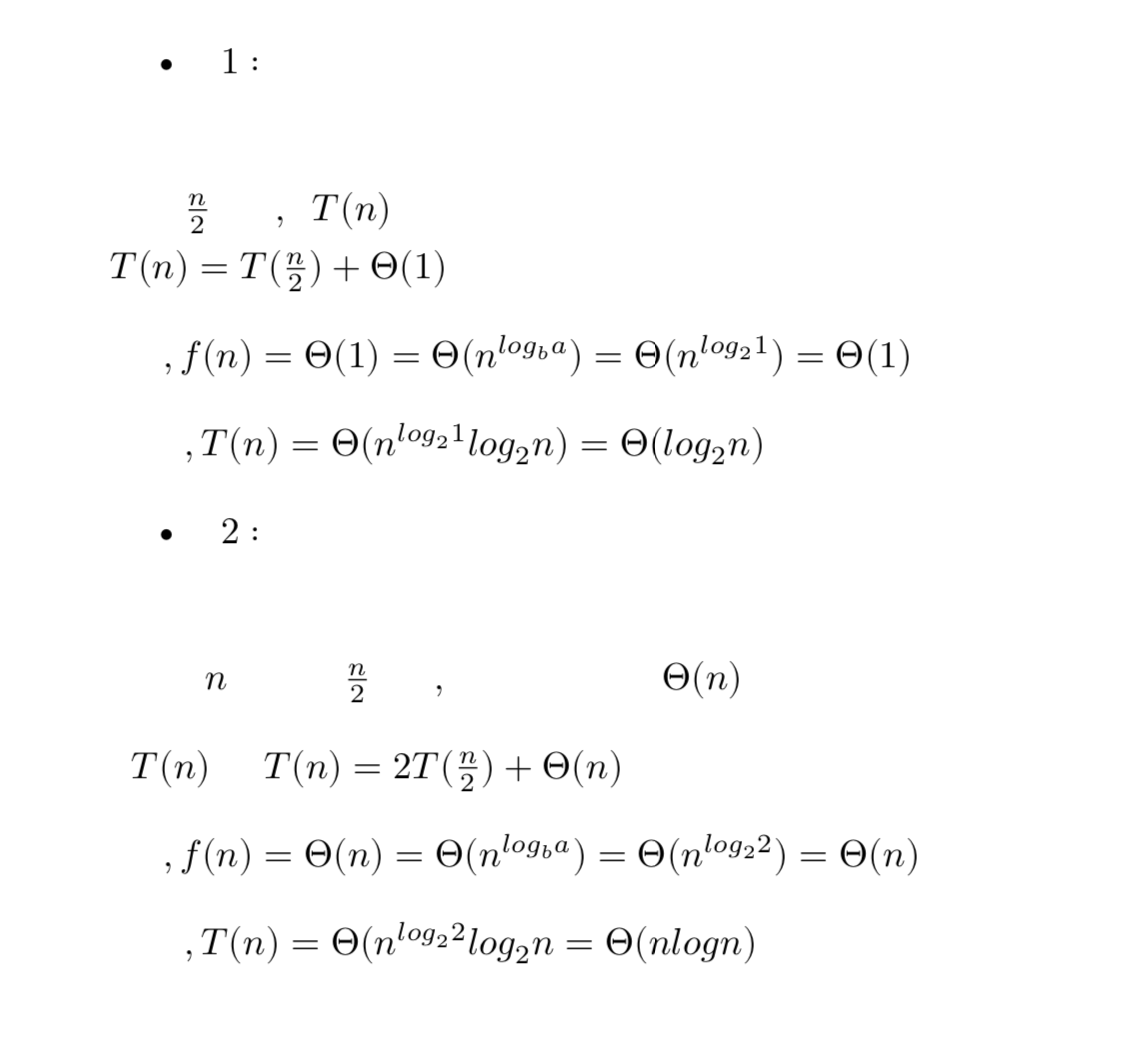
\includegraphics[width=10cm,height=5cm]{image/main1.png}
	\end{minipage}
\end{figure}
\section{主定理的证明}
\begin{figure}[h]
	\begin{minipage}[t]{1\linewidth}
		\centering
		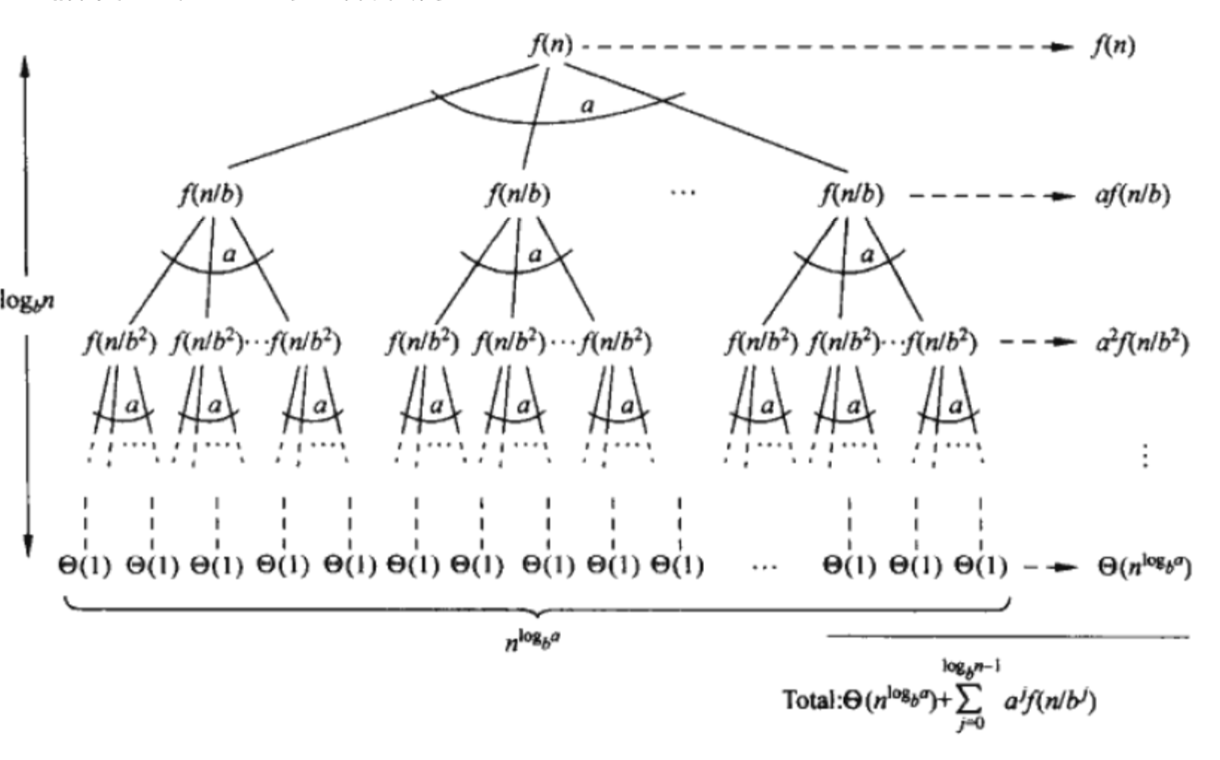
\includegraphics[width=10cm,height=3.5cm]{image/mainmaster.png}
		\caption{递推式展开}
	\end{minipage}
\end{figure}
\subsection{假设 n 是 b 的整数次方}
$T(n)=\Theta\left(n^{\log _{a} b}\right)+\sum_{j=0}^{\log _{b} n-1} a_{j} f\left(n / b^{j}\right)$\\
(1)
 $$
 \begin{array}{l}
f(n)=O\left(n^{l o g_{b} a-\epsilon}\right) \\
g(n)=\sum_{j=0}^{\log _{b} n-1} a_{j} f\left(n / b^{j}\right) \\
f\left(n / b^{j}\right)=O\left(\left(\frac{n}{b^{j}}\right)^{\log _{b} a-\epsilon}\right) \\
c, n_{0}, \forall n \geq n_{0} \\
\left.f\left(n / b^{j}\right) \leq c\left(\frac{n}{b^{j}}\right)^{l o g_{b} a-\epsilon}\right) \Rightarrow a^{j} f\left(n / b^{j}\right) \leq c a^{j}\left(\frac{n}{b^{j}}\right)^{\log _{b} a-\epsilon} \\
a^{j} f\left(n / b^{j}\right) \leq c n^{\log _{b} a-\epsilon}\left(\frac{a}{b^{\log _{b} a-\epsilon}}\right)^{j} \\
\Rightarrow a^{j} f\left(n / b^{j}\right) \leq c n^{\log _{b} a-\epsilon}\left(\frac{a b^{\epsilon}}{b^{\log _{b} a}}\right)^{j} \\
\Rightarrow a^{j} f\left(n / b^{j}\right) \leq c n^{\log _{b} a-\epsilon}\left(b^{\epsilon}\right)^{j} \\
g(n) \leq c n^{\log _{b} a-\epsilon} \sum_{j=0}^{\log _{b} a-1}\left(b^{\epsilon}\right)^{j} \\
\Rightarrow \\g(n) \leq c n^{\log _{b} a-\epsilon} \frac{1\left(1-\left(b^{\epsilon}\right)^{l o g_{b} n}\right)}{1-b^{\epsilon}}
\Rightarrow g(n) \leq c n^{\log _{b} a-\epsilon \frac{1-n^{\epsilon}}{1-b^{\epsilon}}} \\
\Rightarrow g(n) \leq c \frac{n^{\log _{b} a-\epsilon}-n^{\log _{b} a}}{1-b^{\epsilon}} \\
g(n)=O\left(n^{\log _{b} a}\right) \\
T(n)=\Theta\left(n^{\log _{b} a}\right)+O\left(n^{\log _{b} a}\right)=\Theta\left(n^{\log _{b} a}\right)
\end{array}
 $$
